\documentclass[final]{beamer}

\usepackage[
  size=a1,
  orientation=landscape,
  scale=1.5
]{beamerposter}


\usepackage{amsmath,mathtools,amsthm}
\usepackage{amssymb,amsfonts, mathrsfs}
\usepackage{tikz}
\usepackage[dvipsnames]{xcolor}
\usepackage{ragged2e}
\usepackage[normalem]{ulem}
% \usepackage{mlmodern}
\usepackage{quiver}


\usepackage{svg}

% general macros
\newcommand\eqdef{\coloneqq}
\newcommand\nbd{\nobreakdash-\hspace{0pt}}
\newcommand\idd[1]{\mathrm{id}_{#1}}
\newcommand\invrs[1]{#1^{-1}}
\newcommand\after{\circ}

\newcommand\incl{\hookrightarrow}
\newcommand\restr[2]{{#1}{\raisebox{0pt}{$|_{#2}$}}}
\newcommand\powerset[1]{\mathscr{P}{#1}}

\newcommand\set[1]{\left\{ {#1} \right\}}
\newcommand\order[2]{#2^{(#1)}}
\newcommand{\nat}{\mathbb{N}}

% category theory macros

\newcommand\cat[1]{\underline{\mathrm{#1}}}
\newcommand\fun[1]{\mathsf{#1}}
\DeclareMathOperator*{\colim}{colim}
\def\raiseslice#1#2{\raisebox{-2pt}{$#1#2$}}
\newcommand{\slice}[2]{{#1{/}\mathpalette\raiseslice{#2}}}
\newcommand{\counit}{\varepsilon}
\renewcommand{\a}{\alpha}
\newcommand*\cocolon{%
        \nobreak
        \mskip6mu plus1mu
        \mathpunct{}%
        \nonscript
        \mkern-\thinmuskip
        {:}%
        \mskip2mu
        \relax
}

% special categories
\newcommand\rdcpxequal{\cat{rdCpx}}
\newcommand\rdcpxmap{\cat{rdCpx}^{\downarrow}}
\newcommand\rdcpxomega{\rdcpx^{\omega}}
\newcommand\dcpx{\cat{dCpx}}
\newcommand\dcpxomega{\dcpx^{\omega}}
\newcommand\dcpxn[1]{\gr{#1}{\dcpx}}
\newcommand{\dcpxac}{\dcpx^{\mathsf{ac}}}
\newcommand{\Cat}{\cat{Cat}}

\DeclareMathOperator{\Psh}{\cat{Psh}}
\DeclareMathOperator{\sPsh}{\Psh^{\scalebox{0.7}{\( \infty \)}}}
\DeclareMathOperator{\dPsh}{\Psh^{\scalebox{0.7}{\( \Delta \)}}}

\newcommand\Molec{Mol}
\newcommand\Atom{Atom}
\newcommand{\molcat}{\cat{\Molec}}
\newcommand{\atomcat}{\cat{\Atom}}
\newcommand{\atomcatac}{\atomcat^{\mathsf{ac}}
}
\newcommand{\nmolcat}[1]{\gr{#1}{\molcat}}
\newcommand{\natomcat}[1]{\gr{#1}{\atomcat}}

\newcommand\cls[1]{\mathscr{#1}}
\newcommand{\C}{\cls C}

% oriented poset macros
\newcommand\clset[1]{\mathrm{cl}\set{#1}}
\newcommand\gr[2]{#2_{#1}}
\newcommand\maxel[1]{\mathscr{M}\!\mathit{ax}\,#1}
\newcommand\bd[2]{\partial_{#1}^{#2}}
\newcommand\faces[2]{\Delta_{#1}^{#2}}
\newcommand\cofaces[2]{\nabla_{#1}^{#2}}
\newcommand\inter[1]{\mathrm{int}\,#1}
\newcommand\cp[1]{\,{\scriptstyle\#}_{#1}\,}
\newcommand\celto{\Rightarrow}
\newcommand\submol{\sqsubseteq}
\newcommand\sus[1]{\fun{S}{#1}}
\newcommand\maxflow[2]{\mathscr{M}_{#1}{#2}}
\DeclareMathOperator{\frdim}{frdim}

% special shapes
\newcommand{\join}{\,{\star}\,}
\newcommand{\gray}{\otimes}
\newcommand{\ospx}[1]{\vec{\Delta}^{#1}}

% layerings and orderings
\newcommand{\preLay}[1]{\mathscr{P\!L}\!\mathit{ay}_{#1}}
\newcommand{\preOrd}[1]{\mathscr{P\!O}\!\mathit{rd}_{#1}}
\newcommand{\Lay}[1]{\mathscr{L}\!\mathit{ay}_{#1}}
\newcommand{\Ord}[1]{\mathscr{O}\!\mathit{rd}_{#1}}
\renewcommand{\o}[2]{\mathsf{o}_{#1, #2}}

% maps induced
\newcommand{\mapel}[1]{\iota_{#1}}
\newcommand{\imel}[2]{#1_{#2}}
\newcommand{\prt}[1]{\fun{p}_{#1}}

% special objects
\newcommand{\globe}[1]{\vec{O}^{#1}}
\newcommand{\arr}{\vec{I}}
\newcommand{\pt}{1}

% strict functors
\newcommand{\F}{\fun{F}}
\newcommand{\G}{\fun{G}}

% omega cat notations
\newcommand{\nCat}[1]{{\mathsf{s}\Cat_{#1}}}
\newcommand{\omegaCat}{{\mathsf{s}\Cat_{\omega}}}
\newcommand{\somegaCat}{{\mathsf{s}\Cat_{\omega}^>}}
\newcommand{\snCat}[1]{{\mathsf{s}\Cat_{#1}^>}}
\newcommand{\nCatinf}[1]{{\Cat_{#1}}}
\newcommand{\nCatflag}[1]{{\Cat_{#1}^{\mathsf{f}}}}

\newcommand{\strweak}{\iota_{\mathsf{s}}}

\newcommand{\skel}[2]{\gr{\le #1}{#2}}
\newcommand{\N}{\fun{N}}
\newcommand{\locflag}{\mathbb{L}^{\mathsf{f}}}

\newcommand{\pcell}[1]{\langle#1\rangle}
\newcommand\molecin[1]{\slice{\mathit{\Molec}}{#1}}
\newcommand\atomin[1]{\slice{\mathit{\Atom}}{#1}}
\newcommand{\Pd}{\cat{Pd}\,}
\newcommand{\cell}{\cat{cell}\,}

\newcommand{\ThetaS}[1]{\Theta_{#1}}
\newcommand{\Thetan}[1]{\Theta_{#1}}
\newcommand{\ThetanS}[2]{\Theta_{#1, #2}}
\newcommand{\Rtheta}{\fun{R}}
\newcommand{\Utheta}{\fun{U}}

\newcommand{\rs}{\fun{r}^{>}}

% subdivision
\newcommand{\Sd}{\mathrm{Sd}\,}
\newcommand{\Sdi}{\mathrm{Sd}^\triangleleft\,}
\newcommand{\SdS}[1]{\mathrm{Sd}_{#1}}
\newcommand{\SdiS}[1]{\mathrm{Sd}^\triangleleft_{#1}}
\newcommand{\Sdik}[1]{\SdiS{\set{#1}}}
\newcommand{\Sdk}[1]{\SdS{\set{#1}}}
\newcommand{\bigcell}[1]{\mu_{#1}}
\newcommand{\ivl}[2]{[#1,#2]}

% subobject of molecin
\newcommand{\spine}[1]{\fun{sp}_{#1}}
\newcommand{\Spine}{\fun{Sp}\,}
\newcommand{\Smol}{\fun{Qfr}\,}
\newcommand{\sSmol}{\fun{Qfr}_{\scalebox{0.7}{\( < \)}}\,}
\newcommand{\Smolp}{\fun{Qfr}^+\,}
\newcommand{\sSmolp}{\fun{Qfr}^+_{\scalebox{0.7}{\( < \)}}\,}

% regular polygraphs
\newcommand{\Pol}{\cat{regPol}}
\newcommand{\nPol}[1]{\gr{#1}{\Pol}}
\newcommand{\plexcat}{\cat{Plex}}
\newcommand{\polyplexcat}{\cat{polyPlex}}
\newcommand{\nplexcat}[1]{\gr{#1}{\plexcat}}
\newcommand{\npolyplexcat}[1]{\gr{#1}{\polyplexcat}}
\newcommand{\pl}[1]{\underline{#1}}
\newcommand{\posplex}{\Phi}


% ------------------------------------------------------------
% Colors
% ------------------------------------------------------------

\colorlet{cblue}{MidnightBlue}
\colorlet{cgreen}{ForestGreen}
\colorlet{cred}{WildStrawberry}


\colorlet{rblue}{Fuchsia}
\colorlet{rgreen}{ForestGreen}
\colorlet{rred}{BrickRed}
% Useful commands

\newcommand{\blue}[1]{\textcolor{rblue}{#1}}
\newcommand{\red}[1]{\textcolor{rred}{#1}}
\newcommand{\green}[1]{\textcolor{rgreen}{#1}}

\newcommand{\remph}[1]{\textcolor{cblue}{#1}}
\newcommand{\cemph}[1]{\textcolor{cred}{#1}}
\newcommand{\gemph}[1]{\textcolor{cgreen}{#1}}

% ------------------------------------------------------------
% General style
% ------------------------------------------------------------

\setbeamercolor{background canvas}{bg=white}
\setbeamercolor{normal text}{fg=black,bg=white}

\setbeamercolor{block title}{
  fg=rblue,
  bg=white
}

\setbeamercolor{block body}{
  fg=black,
  bg=white
}

\setbeamertemplate{navigation symbols}{}

\setbeamertemplate{itemize item}{
  \small$\blue{\bullet}$
}

\setbeamertemplate{itemize subitem}{
  \scriptsize$\bullet$
}

% Remove block backgrounds and decorations
\setbeamertemplate{block begin}{
  \vspace{1ex}
  {\usebeamerfont{block title}
   \usebeamercolor[fg]{block title}
   \insertblocktitle\par}

  \vspace{0.3ex}

  {\hrule height 1.5pt}

  \vspace{1ex}

  \begin{beamercolorbox}[
    wd=\linewidth,
    sep=0pt
  ]{block body}
}

\setbeamertemplate{block end}{
  \end{beamercolorbox}
  \vspace{1.5ex}
}

% ------------------------------------------------------------
% Fonts
% ------------------------------------------------------------

\setbeamerfont{title}{
  size=\veryHuge,
  series=\sffamily 
}

\setbeamerfont{author}{
  size=\LARGE
}

\setbeamerfont{institute}{
  size=\Large
}

\setbeamerfont{block title}{
  size=\LARGE,
%   series=\bfseries
}

\setbeamerfont{normal text}{
  size=\large
}

% ------------------------------------------------------------
% Poster information
% ------------------------------------------------------------

\title{Diagrammatic $(\infty,n)$-categories}

\author{
  \uline{Cl\'emence Chanavat}
  \qquad
  j.w.w Amar Hadzihasanovic
}

\institute{
  Tallinn University of Technology
}

% ------------------------------------------------------------
% Document
% ------------------------------------------------------------
\usetikzlibrary{nfold}

\setbeamercolor{bibliography entry author}{fg=black}
\setbeamercolor{bibliography entry title}{fg=black}
\setbeamercolor{bibliography entry location}{fg=black}
\setbeamercolor{bibliography entry note}{fg=black}

\begin{document}

\begin{frame}[fragile, t]

% ------------------------------------------------------------
% Title
% ------------------------------------------------------------

\begin{center}

{\usebeamerfont{title}
 \color{rblue}
 {\setlength{\fboxsep}{20pt}\fbox{\parbox{0.60\linewidth}{\centering\inserttitle}}}
 \par}

\vspace{1ex}

{\usebeamerfont{author}
 \insertauthor
 \par}

\vspace{0.5ex}

{\usebeamerfont{institute}
 \insertinstitute
 \par}

\vspace{1ex}

% no line?
% {\hrule height 3pt} 
\begin{tikzpicture}[remember picture,overlay]
  \node[
    anchor=north east,
    xshift=-0cm,
    yshift=-0cm
  ] at (current page.north east) {%
    
\includegraphics[scale=0.2]{img/qr-code.png}%
  };
\end{tikzpicture}
\end{center}

\vspace{-3em}

% ------------------------------------------------------------
% Three columns
% ------------------------------------------------------------

\begin{columns}[t,totalwidth=\textwidth]

% First column
\begin{column}{0.31\textwidth}

\begin{block} {Atom and molecules}
  A \cemph{molecule} is a combinatorial datum encoding the shape of a higher categorical pasting diagram.
  A molecule \( U \):
  \begin{itemize}
    \item is an \cemph{oriented} and graded poset; 
    \item has for each \( \a \in \set{-, +} \) and \( n \in \nat \), a \cemph{input/output \( n \)\nbd boundary}, \( \bd{n}{\a} U \), which is a closed subset of \( U \).
  \end{itemize}
  Molecule can be \cemph{pasted} together: given \( U \), \( V \), and \( n \in \nat \), if \( \bd{i}{+} U \cong \bd{i}{-} V \), then the pushout
  \begin{center}
    \begin{tikzcd}
      {\bd{i}{+} U \cong \bd{i}{-} V} & V \\
      U & {U \cp{k} V}
      \arrow[""{name=0, anchor=center, inner sep=0}, hook, from=1-1, to=1-2]
      \arrow[from=1-1, to=2-1]
      \arrow[from=1-2, to=2-2]
      \arrow[hook, from=2-1, to=2-2]
      \arrow["\lrcorner"{anchor=center, pos=0.125, rotate=180}, draw=none, from=2-2, to=0]
    \end{tikzcd}
  \end{center}
  is a molecule.
  Pasting and boundary of molecules satisfy all the axioms of strict \( \omega \)\nbd categories, and even some \gemph{higher-exchange laws} in dimension \( \geq 4 \).
  An \cemph{atom} is a molecule with a greatest cell.
\end{block}

\vspace{-1em}
\begin{block}{Directed complexes}
    A \cemph{directed complex} \( X \) is a presheaf over the category of atoms.
    It is the combinatorial data to construct a \remph{positive} and \remph{regular} polygraphs:
    \begin{center}
      \begin{tikzcd}
        {\coprod\limits_{u \in \cls S_n} \bd{}{} U} & {\coprod\limits_{u \in \cls S_n} U} \\
        {X_{n - 1}} & {X_n,}
        \arrow[""{name=0, anchor=center, inner sep=0}, hook, from=1-1, to=1-2]
        \arrow["{(\bd{}{}u)_{u \in \cls S_n}}"', from=1-1, to=2-1]
        \arrow["{(u)_{u \in \cls S_n}}", from=1-2, to=2-2]
        \arrow[hook, from=2-1, to=2-2]
        \arrow["\lrcorner"{anchor=center, pos=0.125, rotate=180}, draw=none, from=2-2, to=0]
      \end{tikzcd}
    \end{center}
    There is a construction \( \molecin{X} \) that produces the strict \( \omega \)\nbd category of \remph{molecules in \( X \)}.
    \begin{itemize}
      \item If \( X \) is a graph, \( \molecin{X} \) is the free category on \( X \);
      \item If \( X \) is the \( n \)\nbd dimensional simplex, then \( \molecin{X} \) is the \( n \)\nbd oriental.  
    \end{itemize}
    \red{\uline{Theorem 1.}} under a general acyclicity condition on its molecules, \( \molecin{X} \) is a polygraph, and in fact, a \gemph{weak polygraph}.
\end{block}

\begin{block} {Operations}
  Atom, molecules, and directed complexes, support natively higher categorical operations:
  \begin{itemize}
    \item Gray product \( X \gray Y \),
    \item join \( X \join Y \),
    \item suspension \( \sus{X} \),
    \item duals \( \fun{D}_J X \), where \( J \subseteq \nat \).
  \end{itemize}
\end{block}
\end{column}

% Space between columns
\begin{column}{0.025\textwidth}
\end{column}

% Second column
\begin{column}{0.31\textwidth}

\begin{block}{Examples}

\begin{center}
  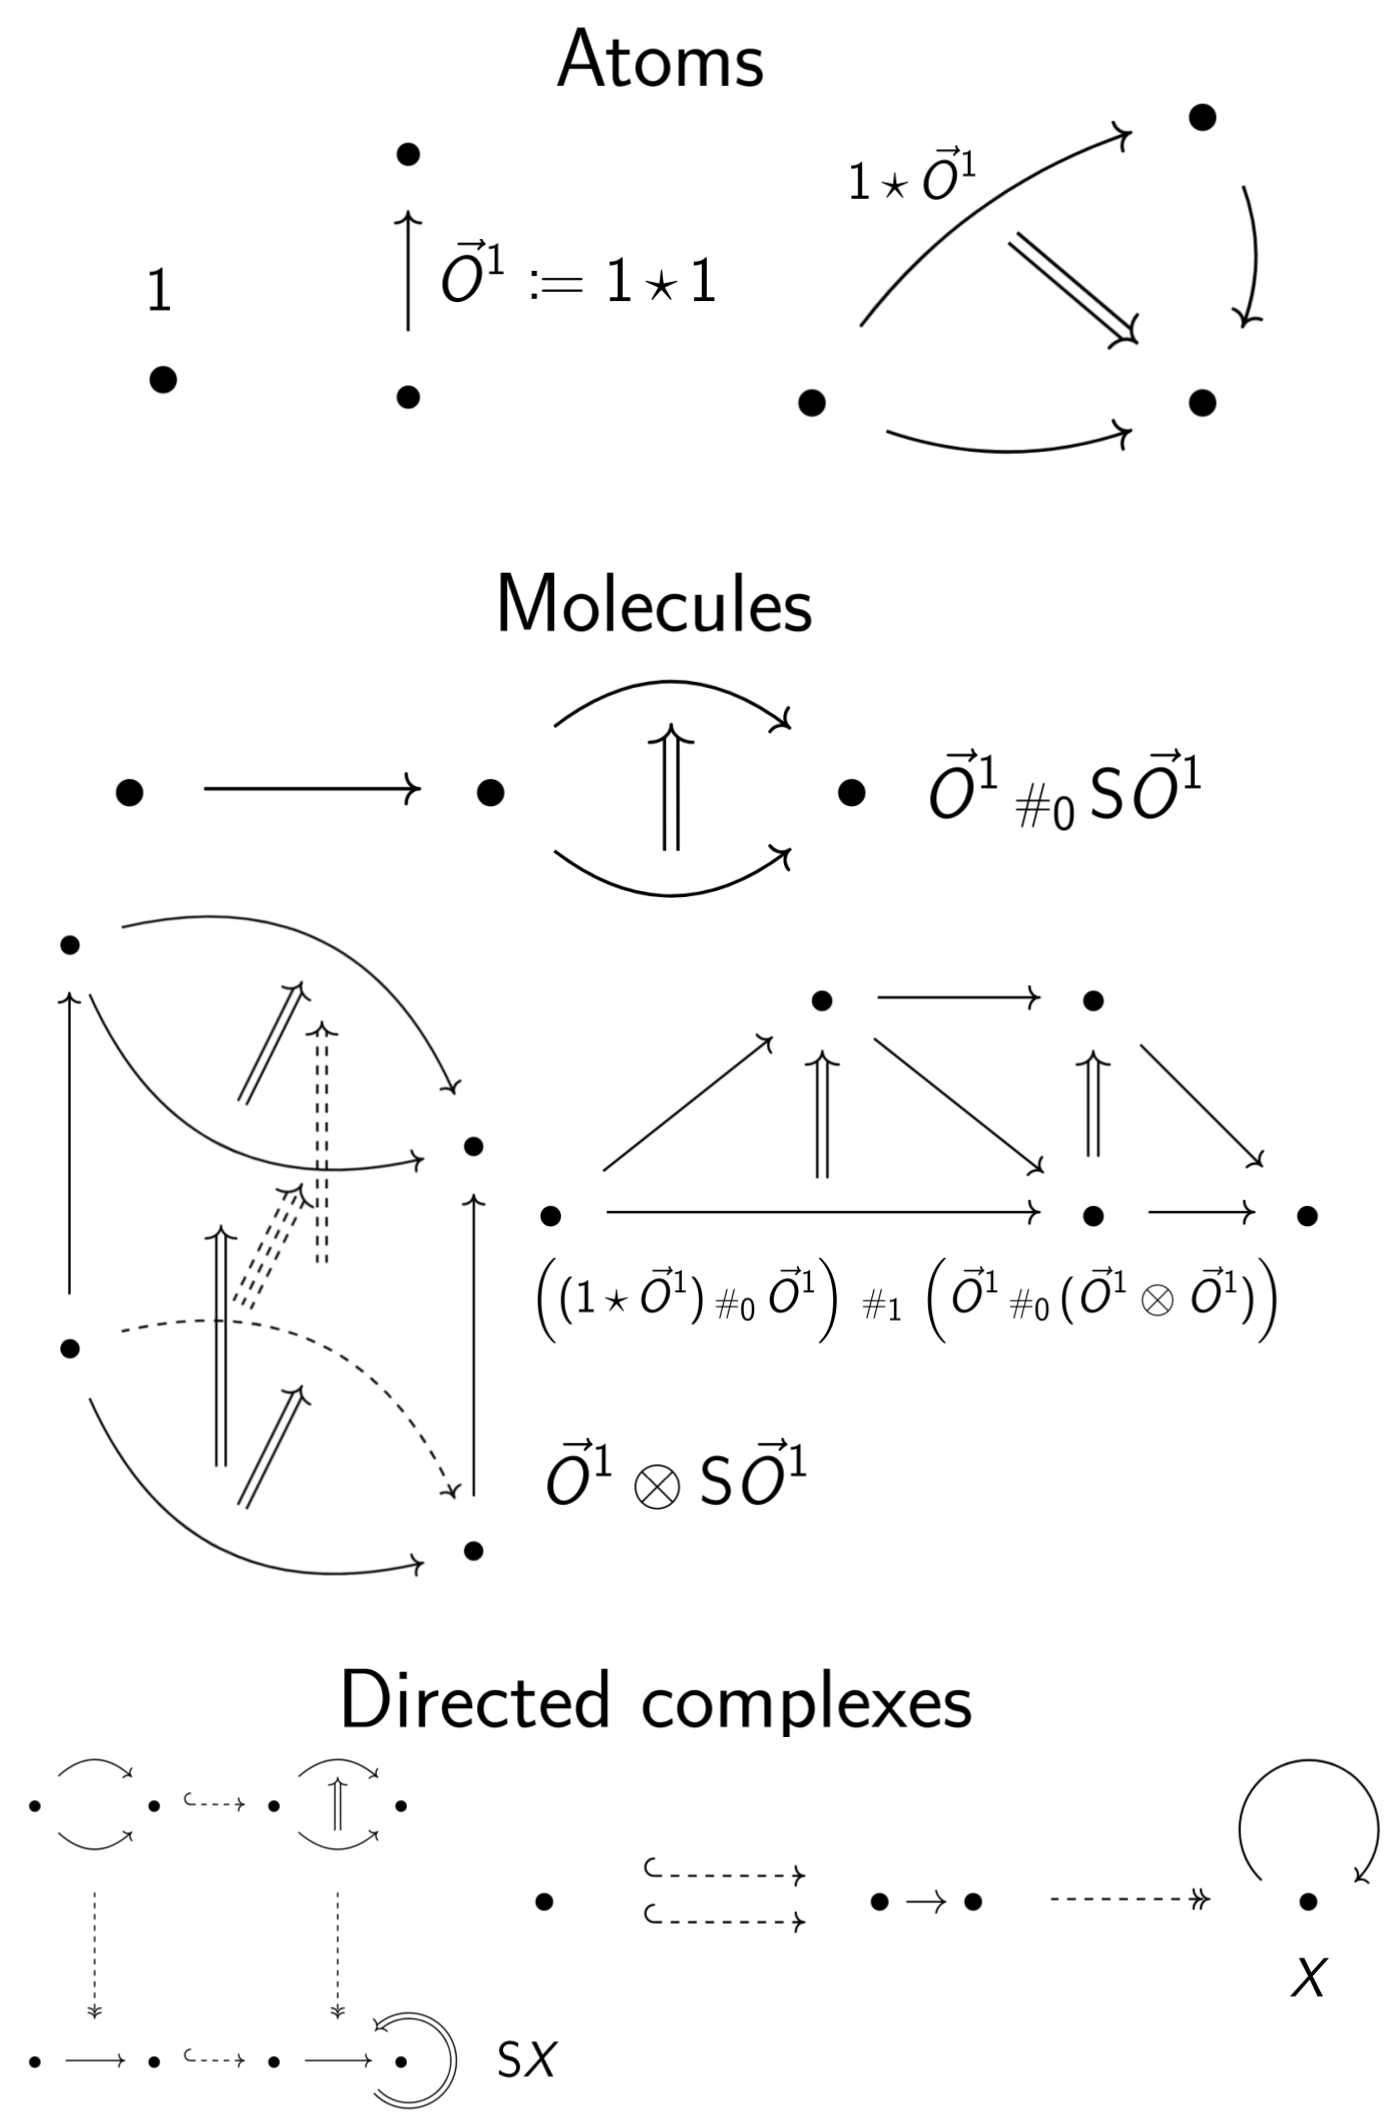
\includegraphics[scale=0.5]{img/exx.png}  
\end{center}
In the last example:
\begin{itemize}
  \item \( \molecin{X} = \fun{B}\nat\)
  \item \( X \) satisfies the acyclicity hypothesis\\ of \red{\uline{Theorem 1.}}
\end{itemize}
  %   {\Large Atoms} \\
%   \vspace{3em}
%   {\Large Molecules} \\
%   \vspace{3em}
%   {\Large Directed complexes} \\
%   \begin{equation*}
%     \pt\quad \globe{1} \eqdef \pt \join \pt\quad \pt \join \globe{1}\quad \globe{1} \cp{0} \sus{\globe{1}}
%   \end{equation*}
%   \begin{equation*}
%     \globe{1} \gray \sus{\globe{1}} \quad \left((\pt \join \globe{1}) \cp{0} \globe{1}\right) \cp{1} \left(\globe{1} \cp{0} (\globe{1} \gray \globe{1})\right)
%   \end{equation*}
%   \vspace{3em}
% \begin{equation*}
%   X \quad \molecin{X} = \fun{B}\nat \quad \sus{X}
% \end{equation*}
% \begin{itemize}
%   \item \( \molecin{X} = \fun{B}\nat\)
%   \item \( X \) satisfies the acyclicity hypothesis\\ of \red{\uline{Theorem 1.}}
% \end{itemize}
\end{block}
\end{column}

% Space between columns
\begin{column}{0.025\textwidth}
\end{column}

% Third columné
\begin{column}{0.31\textwidth}

\begin{block}{Diagrammatic \( (\infty, n) \)\nbd categories}
  Directed complexes may be used in several ways to construct models of \( (0, n) \) and \( (\infty, n) \)\nbd categories:
  \begin{enumerate}
    \item as Segal-sheaves over the \( \molecin{X} \)'s and \remph{strict functors}; 
    \item as presheaves over the atoms and \remph{cellular} strict functors between them;
    A localisation enforces the existence of \cemph{weak composites}.
  \end{enumerate}
  This matches the following two perspective on standard \( (\infty, n) \)\nbd categories as
  \begin{itemize}
    \item Segal-sheaves over the theta's and strict functors;
    \item presheaves over the (marked) orientals and cellular strict functors (i.e. over the marked simplex category).
  \end{itemize}
  \red{\uline{Theorem.}} point \remph{1.} is a localisation of the \( (\infty, n) \)\nbd categories at the higher-exchanges, which does nothing when \( n \le 3 \). \\
  \red{\uline{Conjecture.}} point \remph{1.} and \remph{2.} present the same model of higher-categories.
\end{block}

\begin{block} {Features of the diagrammatic models}
  \begin{itemize}
    \item Very strong \remph{pasting theorems};
    \item \remph{Semi-strictification:} marked directed complexes may be used to two \red{equivalent} model:
    \begin{enumerate}
      \item one where composition is witnessed by \gemph{the existence} of weak composites;
      \item one where composition is \gemph{an operation} satisfying strict associativity and exchange; 
    \end{enumerate}
    In both cases, the unit are algebraic and weak.  
    \item Native support of \remph{higher categorical constructions}, no need to use different presentation.
    \item A rich algebra of \remph{weak units}.
    \item An overall feeling of a \remph{topologically sound alternative} to strict \( n \)\nbd categories
  \end{itemize}
\end{block}
\begin{block}{References}

\small

\begin{thebibliography}{9}

\bibitem{equivalences}
C.~Chanavat and A.~Hadzihasanovic,
\emph{Equivalences in diagrammatic sets},
\newblock Journal of Pure and Applied Algebra, 2026.

\bibitem{reference}
A.~Author,
\newblock \emph{Another reference},
\newblock Journal, year.

\end{thebibliography}

\end{block}

\end{column}

\end{columns}

\end{frame}

\end{document}
